\section{Methods for prediction and analysis of roll damping}
\label{se:methods_for_prediction_and_analysis}
%\subsection{Equations}
%\label{se:equations}
In order to compare the SI-method with data from roll-decay model tests, methods to extract roll damping from tests and the SI-method are first examined. The roll moment along a longitudinal axis though the center of gravity can be expressed according to  \parencite{himeno_prediction_1981} by,

\begin{equation} \label{eq:roll_equation_himeno}
A_{44} \ddot{\phi} + \operatorname{B_{44}}\left(\dot{\phi}\right) + \operatorname{C_{44}}\left(\phi\right) = \operatorname{M_{44}}\left(\omega t\right)
\end{equation}
 

where $A_{44}$ is the total mass moment of inertia, including both ship mass and virtual added mass; $B_{44}$ is the roll damping moment (which is of primary interest in this study) and $C_{44}$ is the restoring moment. $M_{44}$ represents the external moment (usually moment from external waves). For small roll angles, the restoring moments $C_{44}(\phi)$ can be linearized to $C_{1}\phi$. To model the nonlinear restoring moments, $C_{44}(\phi)$ can be described by \emph{n}th order polynomials as $C_{44}(\phi) = C_{1}\phi + C_{2}\phi^2 + C_{3}\phi^3 +, ..., C_{n}\phi^n $
Different experimental test methods are available to determine the coefficients in Eq.(\ref{eq:roll_equation_himeno}). \parencite{ikeda_components_1978} used forced motion tests in which the roll moment was measured for models that were forced to an oscillating roll motion at various frequencies. In this paper, the model scale roll decay tests are used (more information in section \ref{se:database_of_roll_decay_tests}). For these tests the frequency of motion is an output rather than an input (as in the forced motion tests).  Since there are no external forces in such tests, the external moment in Eq.(\ref{eq:roll_equation_himeno}) is zero and the governing equation of the tests becomes, 

\begin{equation} \label{eq:roll_decay_equation_general_himeno}
A_{44} \ddot{\phi} + \operatorname{B_{44}}\left(\dot{\phi}\right) + \operatorname{C_{44}}\phi = 0
\end{equation}



where $B_{44}$ can be expressed as expansion series:  
$ B_{44} = B_1\cdot\dot{\phi} + B_2\cdot\dot{\phi}\left|\dot{\phi}\right| + B_3\cdot\dot{\phi}^3 + ... + B_n\cdot\dot{\phi}^n$. Most often, the so-called ``linear model'', ``quadratic model'' and ``cubic model'' are used to represent $B_{44}(\dot{\phi})$ in Eq.(\ref{eq:roll_decay_equation_general_himeno}) by truncating the series to keep only linear, quadratic and cubic terms,

\begin{equation}
A_{44} \ddot{\phi} + B_{1} \dot{\phi} + \operatorname{C_{44}}\left(\phi\right) = 0
\end{equation}

\begin{equation} \label{eq:roll_decay_equation_himeno_quadratic_b}
A_{44} \ddot{\phi} + C_{1} \phi + \left(B_{1} + B_{2} \left|{\dot{\phi}}\right|\right) \dot{\phi} = 0
\end{equation}

\begin{equation}
A_{44} \ddot{\phi} + \left(B_{1} + B_{2} \left|{\dot{\phi}}\right| + B_{3} \dot{\phi}^{2}\right) \dot{\phi} + \left(C_{1} + C_{3} \left|{\phi}\right| + C_{5} \phi^{2}\right) \phi = 0
\end{equation}



where $B_1$, $B_2$ and $B_3$ are recognized as the roll damping coefficients.
From roll decay tests, those coefficients are normally derived based on the logarithmic decrements of roll peaks. However, this approach is sensitive to low-frequency disturbances and measurement noise. An alternative and more robust approach, which utilizes a full time series of roll decay tests and not just the peaks, is the numerical Parameter Identification Technique (PIT) as described in \parencite{imo_1200_2006} and also used by \parencite{bulian_simplified_2004}. In this approach a numerical solution to a one degree of freedom roll equation is fitted to the roll decay time series by tuning the parameters in the roll equation.

\subsection{Estimation of roll damping from roll decay tests}
\label{se:experimental_estimation}
The roll decay test has the benefit that both roll damping and the natural frequency $\omega_0$ can be observed, but the drawback that roll damping at only this one frequency can be obtained. In order to extract roll damping parameters from the roll decay tests, parameters in the cubic, quadratic or linear roll decay models should be identified. The roll angle is measured during the roll decay tests. The system identification is defined as finding the parameters that produce a simulated roll signal that best fits the roll decay test measurement. 
To evaluate the performed tests, a modified version of the PIT approach is developed. This modified approach adds a time-dependent second-degree polynomial to the fitting. It later can be separated from the solution to account for low frequency disturbances. The roll equation that is used for the evaluation has a linear-quadratic damping dependence and a linear restoring term. 



%Peter Piehl \parencite{henry_peter_piehl_ship_nodate} shows an analytical solution %to the linear model in equation \ref{eq:roll_decay_equation_himeno_linear}, %where the natural frequency of the motion is obtained by:
%\begin{equation}
\omega_{0} = \sqrt{\frac{C}{A_{44}}}
\end{equation}

%
%The roll damping and the natural frequency can be made non dimensional using %the following expressions \parencite{himeno_prediction_1981}: 
%\begin{equation} \label{eq:B44_hat_equation}
B_{44 hat} = \frac{\sqrt{2} \sqrt{\frac{beam}{g}} \operatorname{B_{44}}\left(\dot{\phi}\right)}{2 Disp beam^{2} \rho}
\end{equation}

%\begin{equation} \label{eq:omega_hat_equation}
\omega_{hat} = \frac{\sqrt{2} \omega \sqrt{\frac{beam}{g}}}{2}
\end{equation}

%The ordinary differential equations for roll motion in equation \ref{eq:roll_decay_equation_cubic}, \ref{eq:roll_decay_equation_himeno_quadratic} and \ref{eq:roll_decay_equation_himeno_linear} are solved numerically using Explicit Runge-Kutta method of order 5(4). 

%Figure \ref{fig:analytical} shows a comparison for the linear model between this kind of numerical solution and the exact analytical solution \parencite{henry_peter_piehl_ship_nodate}. It seems that the numerical solution agrees well with the analytical. 

%\begin{figure}[h]
%    \centering
%    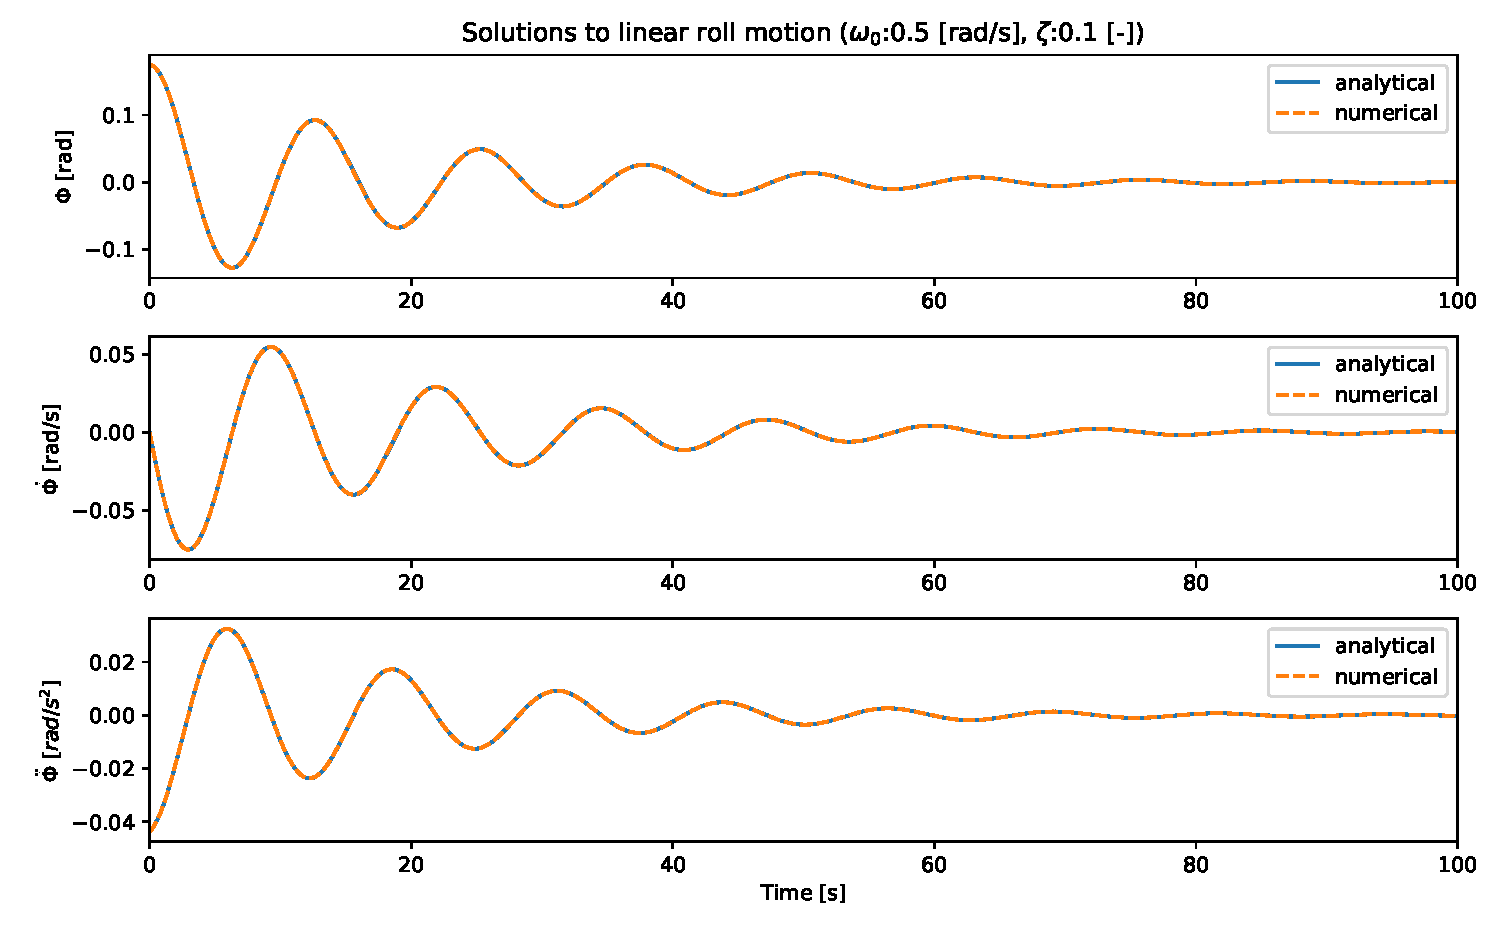
\includegraphics[width=\columnwidth]{figures/analytical.pdf}
%    \caption{Analytical and numerical solution to the linear model}
%    \label{fig:analytical}
%\end{figure}


%\subsection{Parameter Identification Technique}
%\label{se:PIT}
It should be noted that even though the approach could well handle roll equations with higher order of non-linearities in the damping term as well as a non-linear restoring term, the limited amplitudes at which the roll decay tests were conducted cannot motivate advantages of higher order models. 
The goodness of the fit is described using the coefficient of determination:
\begin{equation} \label{eq:R2}
R^2=1-\frac{SS_{res}}{SS_{tot}}
\end{equation}
where $SS_{res}$ is sum of squares of residuals and $SS_{tot}$ is total sum of squares. Two different solution approaches have been investigated for the system identification: a "Derivation approach" and an "Integration approach". 
The "Derivation approach" has the advantage of being very much faster than the "Integration approach" but also the disadvantage of needing to calculate the numerical derivatives which for measurement data also requires some low pass filtration. The "Integration approach" may however also have a disadvantage of not converging.



In the "Derivation approach" the first and second roll time derivatives are calculated numerically so that the parameters in the models are the only unknowns and the optimal parameters that gives the best fit can simply be determined using a least square fit.
In the "Integration approach" the parameters are found by solving a nonlinear least-squares problem using the least-square method \parencite{noauthor_scipyoptimizeleast_squares_nodate} and the Trust Region Reflective algorithm with smooth approximation of l1 (absolute value). This approach requires that ordinary differential equation is solved for many "guessed" sets of parameters till the solution converges.

\begin{figure}[H]
    \centering
    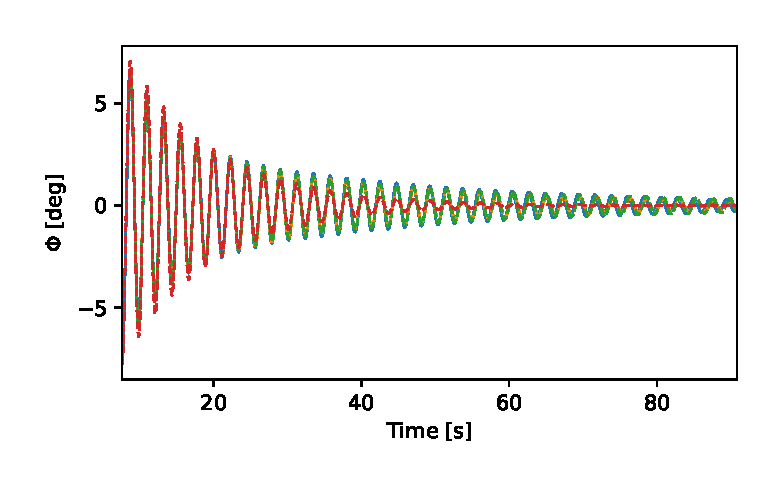
\includegraphics[width=12cm, height = 6cm ]{figures/roll_decay_model_compare.eps}
    \caption{Roll decay test comparison of linear, quadratic and cubic model}
    \label{fig:roll_decay_model_compare}
\end{figure}

A validation of the developed system identification method has been conducted by checking that known parameters from signals from simulations with the linear, quadratic and cubic models can all be identified. For example,
Figure \ref{fig:roll_decay_model_compare} shows a comparison between the linear, quadratic and cubic model for a random chosen roll decay test motion results. It can be seen that the linear model can not give a perfect representation for the whole range of roll angles.    




\subsection{Database of roll decay tests}
\label{se:database_of_roll_decay_tests}

Roll-decay model tests are normally performed prior to other dynamic tests, such as manoeuvring or seakeeping model tests, to check the properties of the tested ship model. In this study, results from such tests, carried out at SSPA in Sweden (www.sspa.se) have been used. The roll-decay tests are conducted by forcing the model to an initial roll angle and then releasing it to oscillate freely in six degrees of freedom. The tests are conducted either  at zero speed or at speed without autopilot. The scaled ship models are from 3 to 6 meters in  length. The measurement accuracy of these model tests is very good. When time series from 20 sets of repeated tests were investigated the average $R^2$ was found to be 0.995. The tests were originally conducted in connection with commercial projects for buildings new merchant ships. In this study, data collected from 2005 to 2018 were used to construct the roll-decay test database, which was applied to build a roll damping database. The ship types in the roll-decay tests used in this paper are  shown in Fig.\ref{fig:ship_types}, and the main parameters of these ships are presented in the sensitivity study as in Fig.\ref{fig:SI_sensitivity}. 


The parameter identification technique was used to estimate the roll damping coefficients from the roll-decay tests. It was investigated whether the linear model Eq.( \ref{eq:roll_decay_equation_himeno_linear}), quadratic model Eq.(\ref{eq:roll_decay_equation_himeno_quadratic_b}) or cubic model Eq.(\ref{eq:roll_decay_equation_cubic}) was best suited to describe the roll damping in all the tests to formulate the roll damping database. After the parameters were identified, the corresponding roll motions were simulated by the three mentioned models. The accuracy of the three models was evaluated with the $R^2$ score coefficient, based on model test and simulation time series of roll motions.
The average $R^2$ was 0.995 for the cubic model, 0.993 for the quadratic, and 0.986 for the linear model. In addition, Fig. \ref{fig:roll_decay_model_compare} shows a comparison between the models for one of the roll-decay tests. It can be seen that the linear model can not give a good representation of the whole range of roll motions, and the difference becomes obvious after the time of 30s. Since the quadratic model has almost the same accuracy as the cubic model it was selected to estimate roll damping from all the roll-decay tests in the database. All the extracted roll damping coefficients together with various ship related information will be formulated as the roll damping database for the following analysis.

\begin{figure}[H]
    \centering
    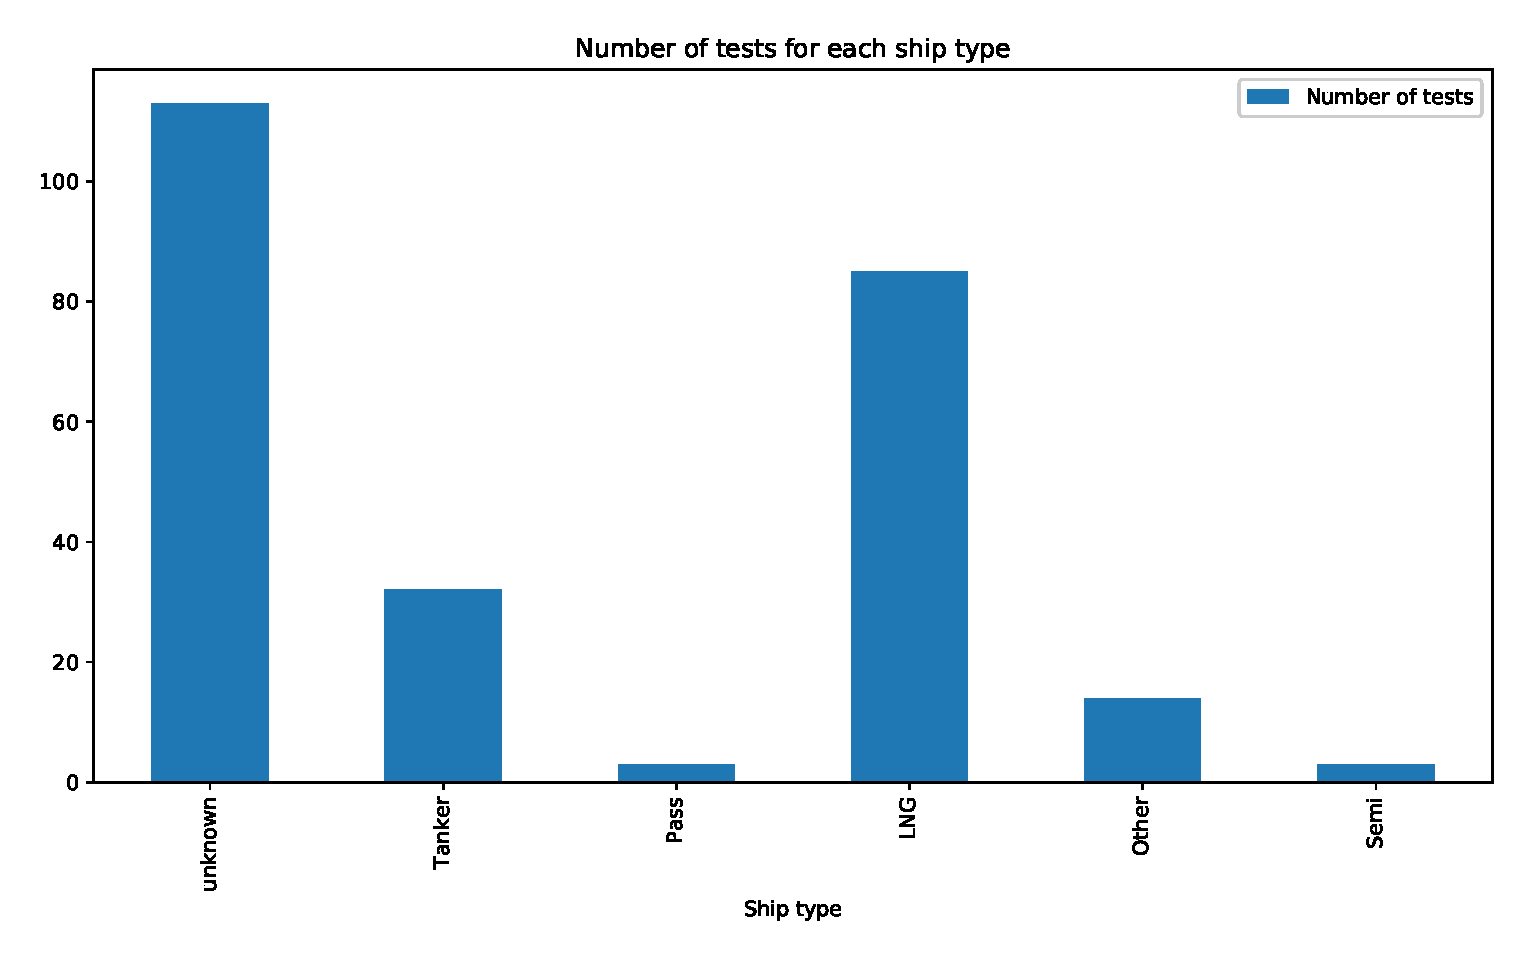
\includegraphics[width=0.5\columnwidth]{figures/ship_types.eps}
    \caption{Number of tests per ship type}
    \label{fig:ship_types}
\end{figure}

\begin{figure}[H]
    \centering
    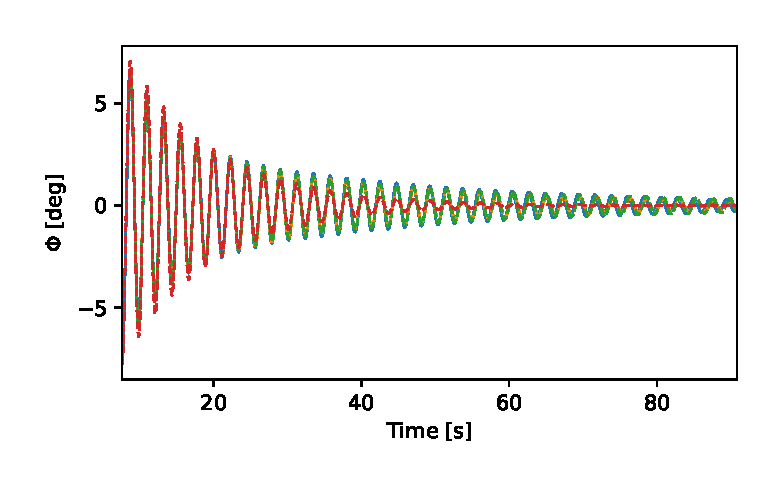
\includegraphics[width=12cm, height = 6cm ]{figures/roll_decay_model_compare.eps}
        \vspace{-0.5cm}
    \caption{Roll-decay test comparison of linear (bottom), quadratic (middle) and cubic model (upper).}
    \label{fig:roll_decay_model_compare}
\end{figure}


\subsection{Ikeda's original method: a strip theory based method}
\label{se:semi-empirical methods}

The roll damping consists of linear and nonlinear components. At zero speed the nonlinear damping is caused by the two-dimensional separation at the bilge keel or near the bilge circle (Eddy damping $B_E$). While at speed the nonlinear damping is mainly caused by the hydrodynamic lift force on the hull, represented as lift damping $B_L$. $B_E$ vanishes at high speed ($F_n>0.15)$ \cite{ikeda_components_1978}.

The wave damping also changes at speed. Ikeda \cite{ikeda_components_1978} proposes a formula for the fraction between wave damping at speed and zero speed: $\frac{B_W}{B_{W0}}$

The Ikeda method has been used to calculate the roll damping for a PCTC vessel Faust \cite{soder_assessment_2019}.


%\begin{figure}[h]
%    \centering
%    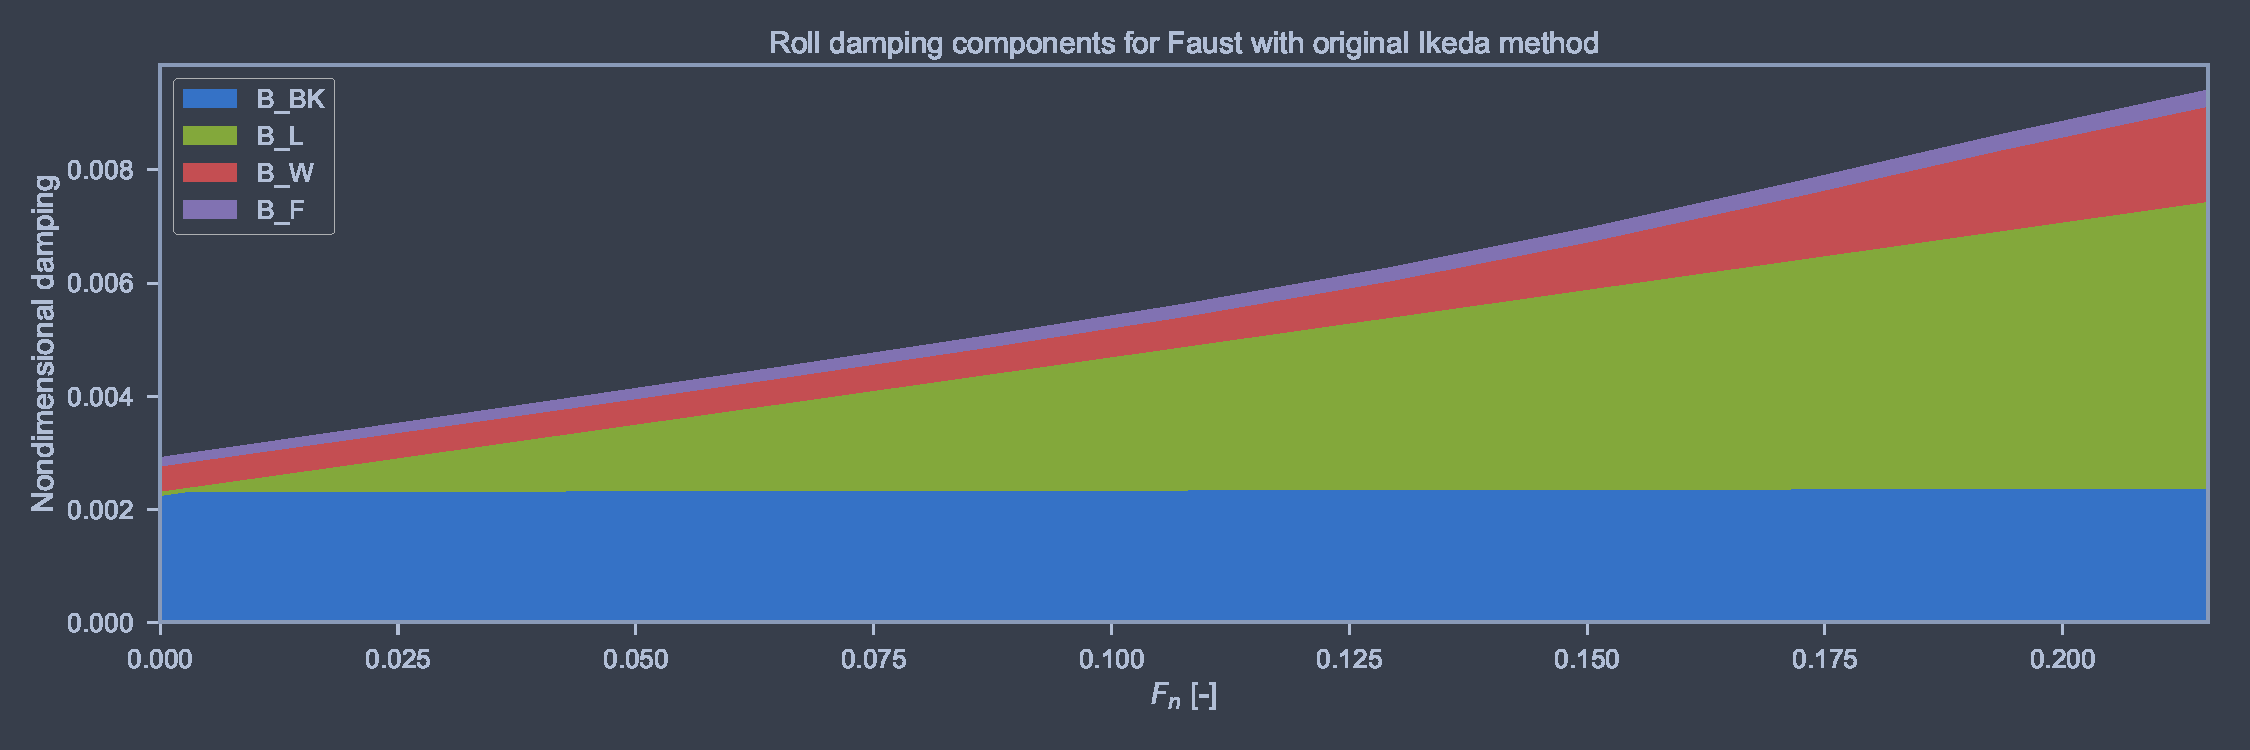
\includegraphics[width=\columnwidth]{figures/ikeda_faust.pdf}
%    \caption{Roll damping components calculated with Ikeda method for PCTC Faust}
%    \label{fig:ikeda_faust}
%\end{figure}



The Ikeda method \cite{ikeda_roll_1978}, \cite{ikeda_eddy_1978}, \cite{ikeda_roll_1979}, \cite{ikeda_components_1978}, \cite{ikeda_velocity_1979} is the most well known semi empirical method to predict roll damping. 

\begin{equation} \label{eq:ikeda}
B = B_F + B_E + B_L + B_W + B_{BK}
\end{equation}

This method divides the roll damping into friction, eddy, lift, waves and bilge keel components (see equation \ref{eq:ikeda}. The wave and eddy components require strip method calculations. This is not an attractive option for the present study since that would require calculations with exact hull geometries to be carried out for all of the ships in the study. There exist however a \emph{Simplified Ikeda method} \cite{kawahara_simple_2011} that is instead used in this study to calculate the eddy component $B_E$ and wave component $B_W$. Figure \ref{fig:ikeda_vs_simplified} shows a comparison between roll damping components calculated with \emph{Ikeda} and \emph{Simplified Ikeda method}. The roll damping is under-predicted with the simplified method for this particular case which is expected according to the limitations of this method  \cite{kawahara_simple_2011}.

\begin{figure}[h]
    \centering
    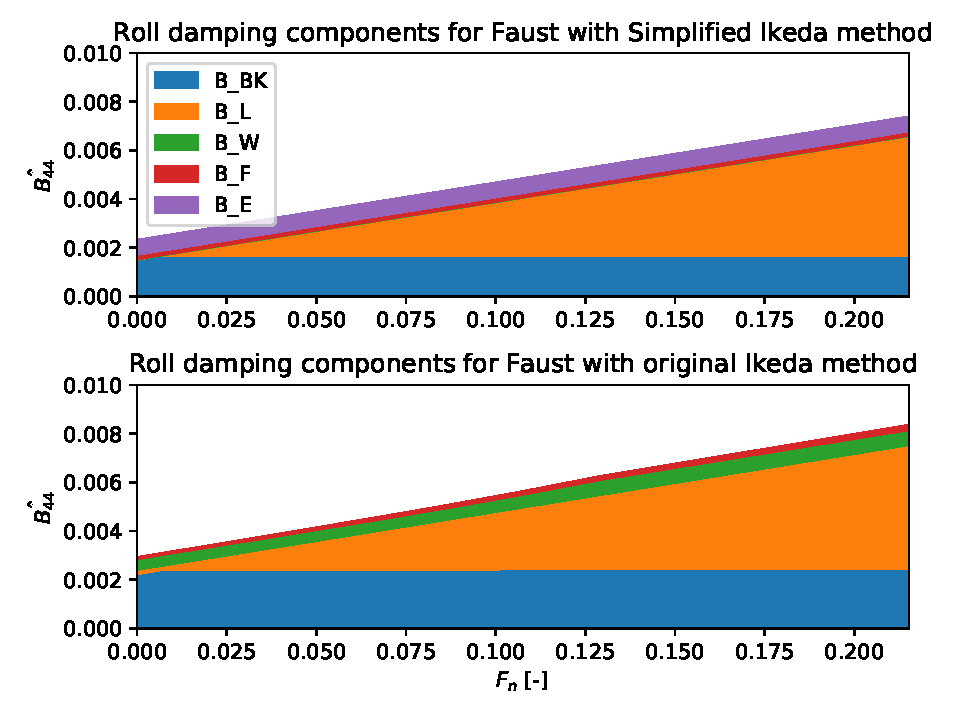
\includegraphics[height=7cm, width=14cm]{figures/ikeda_vs_simplified.pdf}
    \caption{Roll damping components calculated with Ikeda and Simplified Ikeda for PCTC Faust}
    \label{fig:ikeda_vs_simplified}
\end{figure}

